\documentclass[10pt]{report}
\usepackage{./EE703handout}
\usepackage{tikz}
\usepackage{pgfplots}
\usetikzlibrary{decorations.pathmorphing}
\usepackage{mathtools}
\usepackage{subfig}
\usepackage{hyperref}
\usepackage{enumitem}
\usepackage{verbatim}
\usetikzlibrary{arrows,backgrounds,shapes,matrix,positioning,fit}
\setlength{\textheight}{9.4in}     % 9.4in
\setlength{\textwidth}{6.3in}      % 6.3in
\setlength{\parindent}{0mm}
%\setlength{\parskip}{3mm}
\setlength{\oddsidemargin}{0.0in}  % 0.0in
\setlength{\topmargin}{-0.0in}  % 0.0in
\setlength{\headheight}{0.0in}  % 0.0in


\begin{document}
\handout{}{Date: August 27, 2013}{Quiz 1: \textbf{12 points + 3 bonus points}}
The last question will be graded only if the first three questions are answered correctly.
\begin{enumerate}
  \item \textbf{[4 points]} Consider a passband signal $y_p(t)$ centered at $\pm f_c$ given by
    \begin{equation*}
      y_p(t) = \underbrace{\sqrt{2}y_c(t)\cos 2\pi f_c t}_{z_i(t)} - \underbrace{\sqrt{2}y_s(t)\sin 2\pi f_c t}_{z_q(t)}.
    \end{equation*}
  Show that $z_i(t)$ and $z_q(t)$ are orthogonal.
  \item \textbf{[4 points]} Let $p(t) = I_{[0,1)}(t)$ be a pulse of unit amplitude and duration. Find an orthonormal basis for the following signals.
    \begin{eqnarray*}
      s_1(t) & = & p(t) + jp(t-1) \\
      s_2(t) & = & p(t) - jp(t-1) \\
      s_3(t) & = & p(t) + jp(t) \\
    \end{eqnarray*}
    Give the signal space representation of $s_1(t), s_2(t), s_3(t)$ in terms of the orthonormal basis derived.
    \begin{figure}[h]
      \centering
      \begin{tikzpicture}[scale=0.80,transform shape]
        \begin{axis}[
                     title=$p(t)$,
                     xmax=2.0,
                     xmin=0,
                     ymax=1.5,
                     ymin=-0.5,
                     axis lines = middle,
                     ytick={1,0},
                     xtick = {0,1,1.97},
                     xticklabels = {$0$,1,$t$},
                     yticklabels = {1,0},
                    ]
          \addplot[color=blue,very thick] coordinates {(0,1) (1,1) (1,0)};
        \end{axis}
      \end{tikzpicture}
    \end{figure}
  \item \textbf{[4 points]} Consider a random bit $X$ which is equally likely to be 0 or 1. It is passed through a cascade of two binary symmetric channels each having crossover probability $p$. Let the output be $Y$. 
    \begin{enumerate}
      \item What is the probability of $X = 0$ given $Y = 0$?
      \item What is the probability of $X = 1$ given $Y = 0$?
    \end{enumerate}
    \begin{figure}[h]
    \centering
    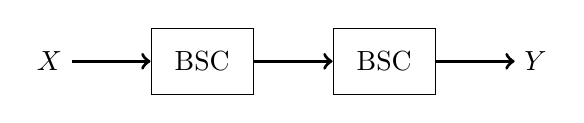
\begin{tikzpicture}[scale=1.0,transform shape]
      \tikzstyle{rectblock}=[rectangle, draw, inner sep=3mm]
      \node (X) {$X$};
      \node[rectblock, right = 1cm of X] (BSC1) {BSC};
      \node[rectblock, right = 1cm of BSC1] (BSC2) {BSC};
      \node[right = 1cm of BSC2] (Y) {$Y$};
      \draw [->,very thick] (X) -- (BSC1);
      \draw [->,very thick] (BSC1) -- (BSC2);
      \draw [->,very thick] (BSC2) -- (Y);
    \end{tikzpicture}
    \end{figure}
  \item \textbf{[3 bonus points]} Give an example of a discrete-time random process which is wide sense stationary but not strict sense stationary.
\end{enumerate}
\end{document}
